\section{Изучение поставленной задачи с помощью\\компьютерного моделирования}

\subsection{Математическая постановка исходной задачи}

Запишем \textbf{общее уравнение непрерывности} в дифференциальной форме:

\begin{equation}\label{eq:main}
\rho_t(\bar{x},t) + div \bar{J}(\bar{x},t) = f(\bar{x},t)
\end{equation}

Оно представляет собой сильную (локальную) форму закона сохранения и выражает связь между потоком $\bar{J} (\bar{x},t)$ и концетрацией (температурой) $\rho(\bar{x},t)$.

Чтобы корректно поставить задачу решения (\ref{eq:main}) необходимо дополнить его ещё одним условием \--- в данной работе оно представлено \textbf{законом диффузии с конвекцией} с отклоняющимся аргументом:

\begin{equation}\label{eq:diffusion-convection}
\bar{J}(\bar{x},t+\tau) = -a^2 \nabla \rho(\bar{x},t) + \bar{V}(\bar{x},t) \rho(\bar{x},t)
\end{equation}

В дальнейшем уравнение (\ref{eq:main}) будет классифицировано с точки зрения теории дифференциальных уравнений с отклоняющимся аргументом. Предварительно приведем необходимую для исследования информацию.

\subsection{Некоторые факты из теории дифференциальных\\уравнений с отклоняющимся аргументом}

\subsubsection{Базовые понятия и определения}

\textbf{Дифференциальными уравнениями с отклоняющимся аргументом} называются дифференциальные уравнения, в которые неизвестная функция и её проиводные входят, вообще говоря, при различных значениях аргумента.

Хотя уравнения с отклоняющимся аргументом по виду очень похожи на обыкновенные дифференциальные уравнения, факт отклонения аргумента усложняет их анализ.

Рассмотрим простейший пример

\begin{equation}\label{eq:example}
\dot{x}(t) = f(t,x(t),x(t-\tau)),
\end{equation}

где $\tau$ \--- положительная константа.

Для начала отметим, что для решения задачи Коши уже недостаточно задать одно начальное условие $x(t_0)=x_0$, ведь необходимо знать исходные значения на всем отрезке $[t_0-\tau,t_0]$, т.е задать функцию $x_0(t)$, определенную на отрезке $[t_0-\tau,t_0]$ \--- \textbf{начальную функцию} (в зарубежной литературе \textbf{history function} или \textbf{initial function}).

\subsubsection{Простейшая модель с запаздыванием}

Для примера рассмотрим две задачи Коши: одну для обыкновенного дифференциального уравнения, другую \--- для уравнения с отклонением по аргументу:

\begin{equation}\label{eq:no-delay}
\left\{
\begin{aligned}
x'(t) = x(t), \quad t>0\\
x(0) = 1
\end{aligned}
\right.
\end{equation}

\begin{equation}\label{eq:delay}
\left\{
\begin{aligned}
y'(t) = y(t-1), \quad t>0\\
y(t) = 1, \quad -1 \leq t \leq 0
\end{aligned}
\right.
\end{equation}

Методы решения подобных уравнений с запаздыванием будут рассмотрены в работе позже, а пока построим графики этих решений:


\begin{figure}
\begin{center}
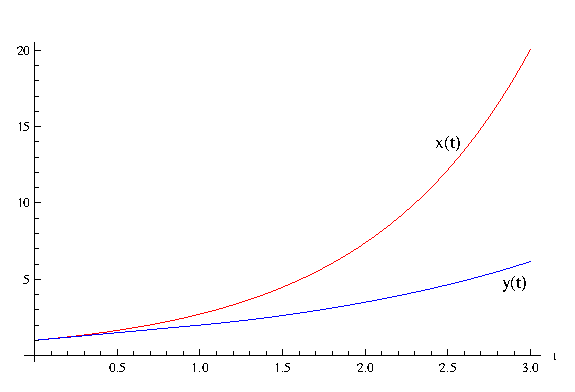
\includegraphics[width=0.65\textwidth]{./1_modelling/comparison.eps}
\end{center}
\caption{Сравнение моделей с запаздыванием и без}
\end{figure}

Наглядно видно, что решения различны. Позже будет приведено аналитическое решение задачи (\ref{eq:delay}) и доказано, что $y(t)$ всегда возрастает медленнее экспоненциального решения, т.е. $x(t)$.

Также решение зависит от начальной функции: для примера рассмотрим такую задачу:

\begin{equation}\label{eq:no-delay-history}
\left\{
\begin{aligned}
y'_h(t) = y_h(t-1), \quad t>0\\
y_h(t) = 1+t, \quad -1 \leq t \leq 0
\end{aligned}
\right.
\end{equation}

Отметим, что $y_h(0) = y(0) = 1$.

Построим решения на одном графике:

\begin{figure}
\begin{center}
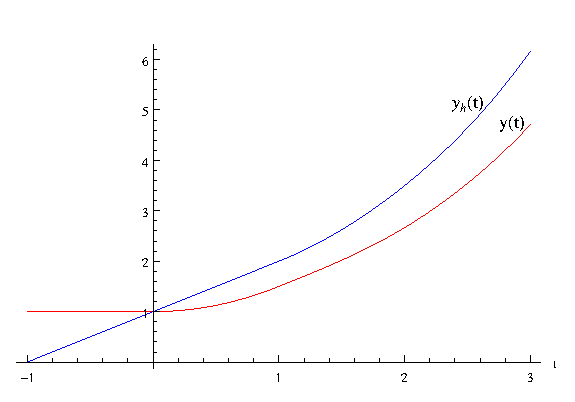
\includegraphics[width=0.65\textwidth]{./1_modelling/comparison_history.eps}
\end{center}
\caption{Сравнение моделей с различными начальными функциями}
\end{figure}

Таким образом, начальная функция определяет характер решения задачи.

\subsubsection{Классификация моделей с отклоняющимся аргументом}

Рассотрим обобщенное уранвнения $n$-ого порядка c $l$ отклонениями аргумента (вообще говоря, отклонение может быть непостоянным и зависеть, например, от значений самого аргумента).

\begin{equation}\label{eq:general-delay}
\begin{aligned}
x^{(m_0)}(t) = f(t,x(t),\dots,x^{(m_0-1)}(t),x(t-\tau_1(t)),\dots,\\\dots,x^{(m_1)}(t-\tau_1(t)),\dots,x(t-\tau_l(t)),\dots,x^{(m_l)}(t-\tau_l(t)))
\end{aligned}
\end{equation}

Здесь $\tau_i(t) \geq 0$.

Каменским Г.А. была введена естественная классификация (\ref{eq:general-delay}). Обозначим $\lambda = m_0 - \max\limits_{1 \leq i \leq l} m_i$.

\begin{enumerate}
\item Если $\lambda > 0$, то такое уравнения называется уравнением с \textbf{запаздывающим аргументом};
\item Если $\lambda = 0$, \--- уравнением \textbf{нейтрального типа};
\item Если $\lambda < 0$, \--- уравнением \textbf{опережающего типа}.
\end{enumerate}

Вернемся к исходной задаче (\ref{eq:main}, \ref{eq:diffusion-convection}):

\begin{equation}
\left\{
\begin{aligned}
\rho_t(\bar{x},t) + div \bar{J}(\bar{x},t) = f(\bar{x},t),\\
\bar{J}(\bar{x},t+\tau) = -a^2 \nabla \rho(\bar{x},t) + \bar{V}(\bar{x},t) \rho(\bar{x},t)
\end{aligned}
\right.
\end{equation}

Объединим в одно уравнение относительно $\rho(x,t)$:

\begin{equation}\label{eq:main-one}
\rho_t(\bar{x},t) = -a^2 \Delta \rho(\bar{x},t-\tau) + \rho(\bar{x},t-\tau) div \bar{V}(\bar{x},t-\tau) + (\bar{V}(\bar{x},t-\tau),\nabla \rho(\bar{x},t-\tau))
\end{equation}

Отметим, что дивергенция как дифференциальный оператор была применена по пространственным переменным $\bar{x}$. Из этого следует, что в левой части (\ref{eq:main-one}) не содержится производных по $t$ и уравнение классифицируется как уравнение с запаздывающим аргументом при $\tau>0$ и как опережающего типа при $\tau<0$.

\subsubsection{Метод шагов решения уравнений\\с отклоняющимся аргументом}

Метод шагов \--- естественный метод решения уравнений с отклоняющимся аргуентом. Рассмотрим простейший пример:

\begin{equation}
x'(t) = f(t,x(t),x(t-\tau)), \quad \tau>0
\end{equation}

Поставим задачу Коши для него:

\begin{equation}\label{eq:delayCauchy}
\left\{
\begin{aligned}
x'(t) = f(t,x(t),x(t-\tau)), \quad t>0,\\
x(t) = x_0(t), \quad -\tau \leq t \leq 0
\end{aligned}
\right.
\end{equation}

Тогда на отрезке $[0,\tau]$:

\begin{equation}\label{eq:toCauchy}
\left\{
\begin{aligned}
x'(t) = f(t,x(t),x_0(t-\tau)), \quad 0 \leq t \leq \tau,\\
x(0) = x_0(0)
\end{aligned}
\right.
\end{equation}

Отметим, что (\ref{eq:toCauchy}) \--- задача Коши уже для обыкновенного дифференциального уравнения. Предположим, что $x_1(t)$ \--- ее решение. Тогда на отрезке $[\tau,2\tau]$:

\begin{equation}\label{eq:toCauchy}
\left\{
\begin{aligned}
x'(t) = f(t,x(t),x_1(t-\tau)), \quad \tau \leq t \leq 2\tau,\\
x(\tau) = x_1(\tau)
\end{aligned}
\right.
\end{equation}

Продолжая подобные рассуждения, можно найти решение (\ref{eq:delayCauchy}). Отметим, что решать можно как аналитически, так и численно.

К минусам этого метода можно отнести зависимость от величины отклонения и сложность адаптации к общему случаю зависимости запаздывания от аргумента.

В качестве примера можно рассмотреть уже использованную раннее в работе задачу Коши (\ref{eq:delay}):

\begin{equation*}
\left\{
\begin{aligned}
y'(t) = y(t-1), \quad t>0\\
y(t) = 1, \quad -1 \leq t \leq 0
\end{aligned}
\right.
\end{equation*}

Таким образом, на отрезке $[0,1]$ её решением будет функция

\begin{equation}
y(t) = t+1, \quad 0 \leq t \leq 1
\end{equation}

На отрезке $[1,2]$ соответственно:

\begin{equation}
\left\{
\begin{aligned}
y'(t) = (t+1)-1, \quad 1 \leq t \leq 2,\\
y(1) = 1 + 1 = 2
\end{aligned}
\right.
\end{equation}

\begin{equation}
y(t) = \dfrac{t^2}{2} + \dfrac{3}{4}, \quad 1 \leq t \leq 2
\end{equation}

Продолжая подобные рассуждения, можно построить решение на сколь угодно отдаленном по времени от начального момента отрезке.

Заметим, что на каждом из таких отрезков, решения представлены в виде полинома, а значит возрастают не быстрее решения задачи без запаздывания \--- экспоненциальной функции.

\subsubsection{Некоторые сведения о решениях линейных уравнений\\с постоянными коэффициентами и постоянными\\отклонениями аргумента}
Рассмотрим линейное однородное уравнение с постоянными коэффициентами и постоянными отклонениями аргумента

\begin{equation}\label{eq:generalized-delay}
\sum\limits_{i=0}^{n} \sum\limits_{j=0}^{l} a_{ij} x^{(i)}(t-\tau_j) = 0,
\end{equation}

где $0=\tau_0 < \tau_1 < \dots < \tau_m$.

Будем искать его частные решения в виде

\begin{equation}\label{eq:partial-delay}
x(t) = e^{kt},
\end{equation}

где $k$ \--- постоянная.

Подставив (\ref{eq:partial-delay}) в (\ref{eq:generalized-delay}), получим характеристическое уравнение для $k$:

\begin{equation}\label{eq:characteristic-delay}
\sum\limits_{i=0}^{n} \sum\limits_{j=0}^{l} a_{ij} k^i e^{k \tau j} = 0
\end{equation}

Теория подобных трансцедентных уравнений изучалась ещё в $XVIII$ веке Ламбертом и Эйлером. Известно, что (\ref{eq:characteristic-delay}) имеет бесконечное множество корней в комплексном пространстве.

В честь немецкого математика Ламберта была названа функция $W(z)$, определяемая функциональным уравнением

\begin{equation}
z = W(z) e^{W(z)}
\end{equation}

Вообще говоря, $W(z)$ многозначна, но если ограничиться вещественными $z = x \geq -\frac{1}{e}$ и потребовать $W(z) \geq -1$, то получим однозначно определенную функцию, представляющую одну из главных ветвей $W(z)$:

\begin{figure}
\begin{center}
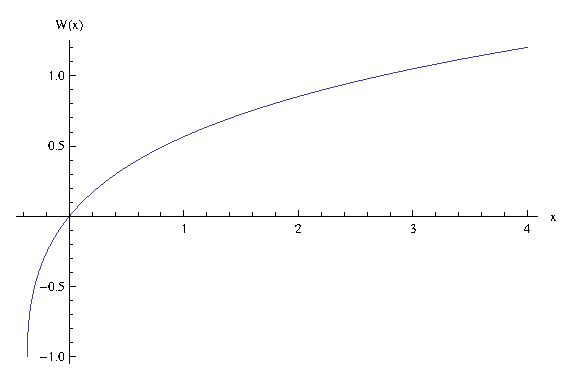
\includegraphics[width=0.65\textwidth]{./1_modelling/Lambert.eps}
\end{center}
\caption{График главной ветви $W_0(x)$ решений функции Ламберта}
\end{figure}

\subsection{Переход к исследованию обыкновенных\\уравнений в частных производных,\\приближающих исходное уравнение\\с запаздыванием}

Цель дальнейшего исследования \--- свести исходную задачи к анализу её приближений уравнениями в частных производных.

Напомним, что в работе исследуется задача (\ref{eq:main}, \ref{eq:diffusion-convection}):

\begin{equation}
\left\{
\begin{aligned}
\rho_t(\bar{x},t) + div \bar{J}(\bar{x},t) = f(\bar{x},t),\\
\bar{J}(\bar{x},t+\tau) = -a^2 \nabla \rho(\bar{x},t) + \bar{V}(\bar{x},t) \rho(\bar{x},t)
\end{aligned}
\right.
\end{equation}

Разложим левую часть уравнения с запаздыванием в ряд Тэйлора, опустив члены порядка выше $m$:

\begin{equation}
\bar{J}(\bar{x},t) + \bar{J_t}(\bar{x},t) \tau + \dots + \dfrac{\partial^m \bar{J}}{\partial t^m}(\bar{x},t) \dfrac{\tau^m}{m!} = -a^2 \nabla \rho(\bar{x},t) + \bar{V}(\bar{x},t) \rho(\bar{x},t)
\end{equation}

\begin{equation}\label{eq:sub}
\sum\limits_{n=0}^{m} \dfrac{\partial^n \bar{J}}{\partial t^n}(\bar{x},t) \dfrac{\tau^n}{n!} = -a^2 \nabla \rho(\bar{x},t) + \bar{V}(\bar{x},t) \rho(\bar{x},t)
\end{equation}

В контексте работы будем называть $m$ \textbf{порядком приближения}.

Продифференциировав (\ref{eq:main}) $n$ раз, получим:

\begin{equation}
\dfrac{\partial^{n+1} \rho}{\partial t^{n+1}} + div \dfrac{\partial^n \bar{J}}{\partial t^n} = \dfrac{\partial^n f}{\partial t^n}
\end{equation}

Домножив последнее уравнение на $\frac{\tau^n}{n!}$, перепишем его в следующем виде:

\begin{equation}\label{eq:div}
div \left( \dfrac{\partial^n \bar{J}}{\partial t^n} \right) \dfrac{\tau^n}{n!} = \left(\dfrac{\partial^n f}{\partial t^n} - \dfrac{\partial^{n+1} \rho}{\partial t^{n+1}} \right) \dfrac{\tau^n}{n!}
\end{equation}

Из уравнения (\ref{eq:sub}):

\begin{equation}
\sum\limits_{n=0}^{m} div \left(\dfrac{\partial^n \bar{J}}{\partial t^n} \right) \dfrac{\tau^n}{n!} = -a^2 div(\nabla \rho) + div(\bar{V} \rho)
\end{equation}

Подставим (\ref{eq:div}):

\begin{equation}
\sum\limits_{n=0}^{m} \left(\dfrac{\partial^n f}{\partial t^n} - \dfrac{\partial^{n+1} \rho}{\partial t^{n+1}} \right) \dfrac{\tau^n}{n!} = - a^2 \Delta \rho + \rho div\bar{V} + (\bar{V},\nabla \rho)
\end{equation}

\begin{equation}
\sum\limits_{n=0}^{m} \dfrac{\partial^{n+1} \rho}{\partial t^{n+1}} \dfrac{\tau^n}{n!} - a^2 \Delta \rho + \rho div\bar{V} + (\bar{V},\nabla \rho) = \sum\limits_{n=0}^{m} \dfrac{\partial^n f}{\partial t^n} \dfrac{\tau^n}{n!}
\end{equation}

Рассмотрим одномерный случай:

\begin{equation}
\sum\limits_{n=0}^{m} \dfrac{\partial^{n+1} \rho}{\partial t^{n+1}} \dfrac{\tau^n}{n!} - a^2 \dfrac{\partial^2 \rho}{\partial x^2} + \rho \dfrac{\partial V}{\partial x} + V \dfrac{\partial \rho}{\partial x} = \sum\limits_{n=0}^{m} \dfrac{\partial^n f}{\partial t^n} \dfrac{\tau^n}{n!} = g(x,t)
\end{equation}

Для простоты примем $g=0$ и $V=const$:

\begin{equation}
\sum\limits_{n=0}^{m} \dfrac{\partial^{n+1} \rho}{\partial t^{n+1}} \dfrac{\tau^n}{n!} - a^2 \dfrac{\partial^2 \rho}{\partial x^2} + V \dfrac{\partial \rho}{\partial x} = 0
\end{equation}

Заменим неизвестную функцию следующим образом:

\begin{equation}
\rho (x,t) = e^{\xi x} u(x,t)
\end{equation}

Тогда

\begin{align}
\rho_x & = e^{\xi x} (u_x + \xi u)\\
\rho_{xx} & = e^{\xi x} (u_{xx} + 2 \xi u_x + \xi^2 u)
\end{align}

\begin{align}
- a^2 \rho_{xx} + V \rho_x = e^{\xi x} \lbrack -a^2 (u_{xx} + 2 \xi u_x + \xi^2 u) + V (u_x + \xi u) \rbrack = \\
= e^{\xi x} \lbrack -a^2 u_{xx} + (-2 a^2 \xi + V) u_x + (-a^2 \xi^2 + V \xi) u \rbrack = \\
= e^{\xi x} \left\lbrack -a^2 u_{xx} + \dfrac{V^2}{4a^2} u \right\rbrack
\end{align}

при $\xi = \frac{V}{2a^2}$ (т.е. коэффициент при $u_x$ равен $0$).

Наконец, получим уравнение, для которого будем исследовать устойчивость его решений:

\begin{equation}\label{eq:final-n}
\sum\limits_{n=0}^{m} \dfrac{\partial^{n+1} u}{\partial t^{n+1}} \dfrac{\tau^n}{n!} - a^2 \dfrac{\partial^2 u}{\partial x^2} + \dfrac{V^2}{4a^2} u = 0
\end{equation}

Для уравнения \ref{eq:final-n} применим \textbf{метод Фурье разделения переменных}:

\begin{equation}
u(x,t) = \sum\limits_{k=1}^{\infty} X(x)T(t)
\end{equation}

Получим:

\begin{equation}
\sum\limits_{n=0}^{m} \dfrac{\tau^n}{n!} T^{(n+1)} X + \dfrac{V^2}{4a^2} T X =a^2 T X'', \quad k=1,\dots,\infty
\end{equation}

\begin{equation}
\dfrac{\sum\limits_{n=0}^{m} \dfrac{\tau^n}{n!} T^{(n+1)} + \dfrac{V^2}{4a^2} T}{a^2 T} = \dfrac{X''}{X} = -\lambda = -k^2
\end{equation}

\begin{equation}
\left\{
\begin{aligned}
\sum\limits_{n=0}^{m} \dfrac{\tau^n}{n!} T^{(n+1)} + \underbrace{ \left( \dfrac{V^2}{4a^2} + a^2 k^2 \right)}_{\gamma(k^2)} T & = 0\\
X'' + k^2 X & = 0
\end{aligned}
\right.
\end{equation}

Как видно, малый параметр входит только в уравнение относительно $T(t)$.

Дальнейшей целью настоящего исследования станет вопрос об устойчивости нулевого решения

\begin{equation}
\sum\limits_{n=0}^{m} \dfrac{\tau^n}{n!} T^{(n+1)} + \underbrace{ \left( \dfrac{V^2}{4a^2} + a^2 k^2 \right)}_{\gamma(k^2)} T = 0
\end{equation}

при различных $m$.